\documentclass[oneside,a4paper,12pt]{article}
\usepackage{graphicx}
\usepackage{amsmath}
\usepackage{listings}
\lstset{language=html}
\usepackage{array}
\usepackage{pdfpages}
\usepackage{biblatex}
\addbibresource{rapport.bib}
\usepackage{hyperref}
\graphicspath{{~/templates/}, {../images/}}

\makeindex
\begin{document}
	\begin{titlepage}
		\includegraphics[width=4cm]{logopopo.png}
		\hspace*{\fill}
		\includegraphics[width=6cm]{logouniv.png}
		
		\begin{center}
			\vspace{1cm}
			\textbf{Compte rendu technique}\\
			\vspace{1cm}
			\textbf{\LARGE 3D Printing Loop}\\
			\textbf{\large Du concept à la réalité}\\
			\vspace{10cm}
			\textbf{Maxence NEUS}\\
			
			\vspace{\fill}
			\textbf{2023}\\
		\end{center}
	\end{titlepage}
	
	\tableofcontents
	\newpage
	
	\section{Introduction}
	
	
	
	\section{Préparation des models}
	
	Pour pouvoir imprimer les models de plantes générés, on a besoin de les préparer. En effet les géométries générées comportent des pièces flottantes qui ne sont pas ratachées au reste du model.
	
	Le processus de préparation consiste en deux étapes :
	\begin{itemize}
		\item[1.] Sous Meshlab on supprime la majorité des pièces flottantes avec un outil intégré qui supprime les groupes de points d'une taille donnée qui sont indépendants
		\item[2.] Sous Bender on sculpte le model aux endroits où Meshlab n'a pas supprimé suffisament de matériau et on ajoute des supports "organiques" là où c'est possible
	\end{itemize}
	
	\section{Impression 3D}
	
	D'abord on a décidé de l'imprimante qui sera utilisée pour l'accrochage final: nous avons choisi la Crrality Ender3 Pro pour son faible coût et sa bonne fiabilité en plus du bon support de la communauté qui devrait aider Thomas à rêgler les potentiels problèmes par la suite.
	
	\subsection{Tests des models}
	
	Dans un premier temps et pour valider la faisabilité de l'impression on a voulu tester quelques models pour observer la qualité de l'impression.
	
	On a utilisé un slicer basé sur Slic3r (\href{https://github.com/RotBotSlicer/Transform}{SuperSlicer}) qui nous permet de placer manuellement les supports d'impression plutôt que de laisser le slicer le faire automatiquement, ce qui nous permet de contrôler l'apparance du model pendant l'impression.
	
	\begin{figure}[h]
		\centering
		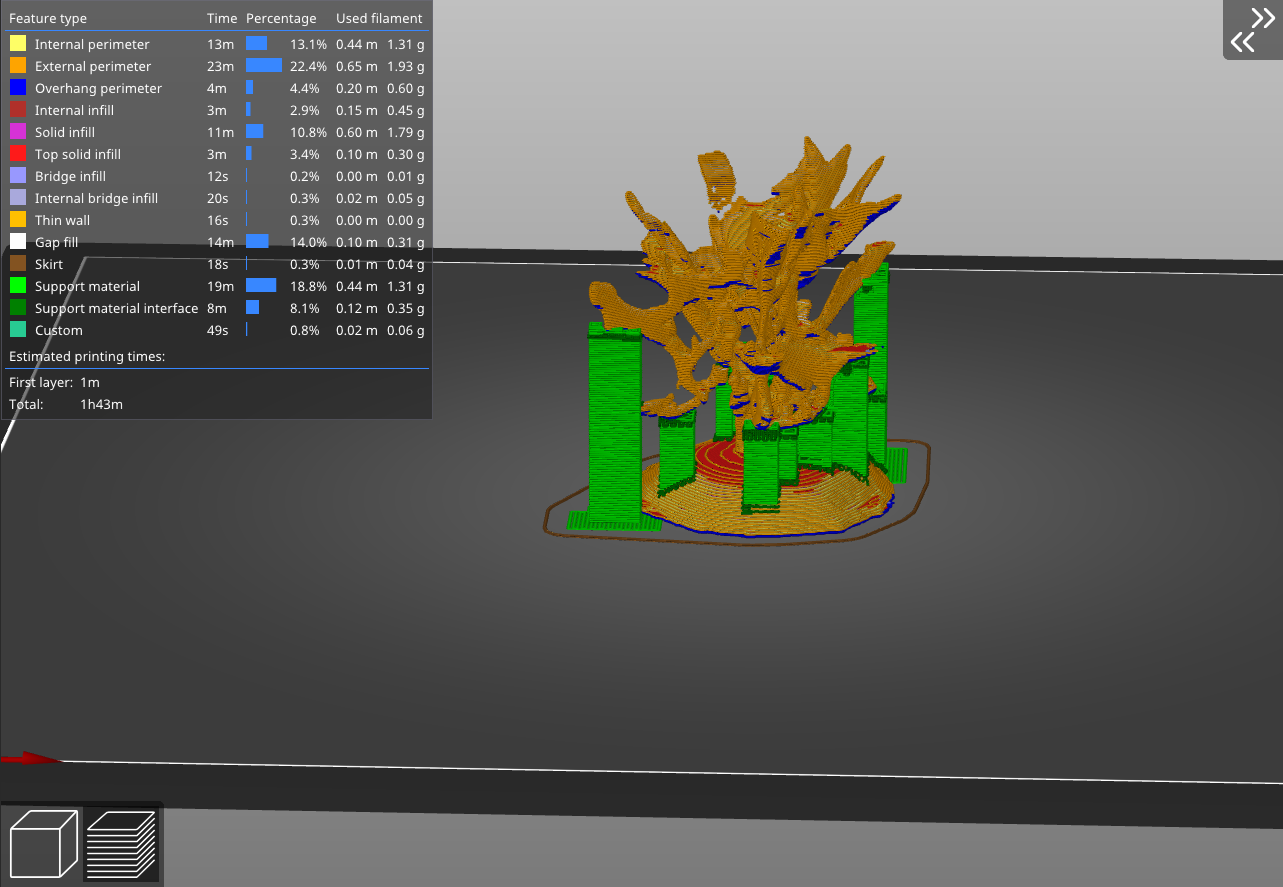
\includegraphics[width=10cm]{superslicer.png}
		\caption{Model du slicer}	
	\end{figure}
	
	\subsection{Impression en continu}
	
	Le projet demande d'imprimer les models en continu. C'est à dire que lorsqu'une impression se termine, on doit retirer le model de l'imprimante afin de libérer la place pour le suivant.
	
	Pour cela on a choisis d'implémenter une technique créée pendant la période du début de pandémie pour imprimer des "face shields" pour les hôpitaux. Cette technique consiste à modifier légerement le Gcode en fin de programme pour supprimer la procédure de fin et y insérer à la place le code suivant :
	
	\begin{figure}[h]
		\centering
		\begin{lstlisting}
; 1:
G91 ; Coordonnees relatives
G1 Z5 ; 

; 2:
G90 ; Coordonnees absolues
G1 X130 Y230 Z5

; 3:
G28 Y ; Auto Home l'axe Y

; 4:
G0 Y230 F2000
		\end{lstlisting}
		\caption{Code de fin d'impression}
	\end{figure}
	
	Ce code permet de :
	\begin{itemize}
		\item[1] soulever la tête d'impression de quelques millimètres de la pièce pour s'assurer de ne pas rentrer dedans lors de la prochaine étape.
		\item[2] Déplacer la tête derrière le model 
		\item[3] Auto Home l'axe Y pour ramener la tête à l'avant du plateau, décollant ainsi le model avec l'axe X de l'imprimante
		\item[4] Ramener le plateau à l'avant pour faire tomber le model maintenant positionné juste devant le plateau vers l'avant de l'imprimante 
	\end{itemize}
	
	Notre test initial avec un model de simple cube a été très fructueux, le model se décollant aisément du plateau. Notre second test avec le model présenté en 3.1 n'as pas été fructueux, en effet l'adhérence de ce model est trop grande pour les moteurs de l'imprimante qui ne parviennent pas à le décoller.
	Pour rêgler ce problème, on propose d'ajouter un raft au model afin d'avoir une surface d'adhésion moindre mais qui permette toujours d'obtenir une qualité d'impression suffisante.
	
	\section{Station de recyclage}
	
	\subsection{Implémentation artistique}
	
	\subsubsection{Choix technique}
	La solution étudiée en Annexe B apporte un co\`ut trop important qui ne peut pas être ammorti par les fonds accordés à PRIST, on propose donc une implémentation plus narrative pour l'oeuvre.
	Pour émuler l'extrusion de plastique, on propose de dérouler une bobine pleine à travers un orifice qui simule une buse d'extrusion sur une bobine vide.
	
	Pour cela on a besoin de motoriser la bobine vide pour qu'elle puisse dérouler le fillament. On propose une solution simple et résiliente qui consiste à découper des engrenages à la découpeuse laser que l'on va fixer à la bobine et à un moteur.
	
	\subsubsection{Dimensionement}
	Pour obtenir un effet plus réaliste, la bobine doit tourner assez lentement pour coller à une vitesse d'extrusion du plastique réaliste. On cherche donc a avoir un rapport de réduction de la chaîne d'engrenages le plus grand possible.
	
	On utilise les outils d'Onshape pour créer deux engrenages pour la bobine et le moteur, en expérimentant avec l'outil on a choisit un module de 1.5mm qui correspond à une limite pratique de la découpeuse laser (un module plus faible donnerait des engrenages brulés au niveau des dents ce qui ne permettrait pas un engrainement correct). Pour coller aux dimensions de la bobine, on choisit un engranage à 120 dents pour la bobine (qui donne un diametre de 180 mm) et un de 20 dents pour le moteur (pour un diametre de 20 mm).
	
	On obtient donc un rapport de réduction de $ \frac{20}{120} = 1:6 $
	
	\begin{figure}[h]
		\centering
		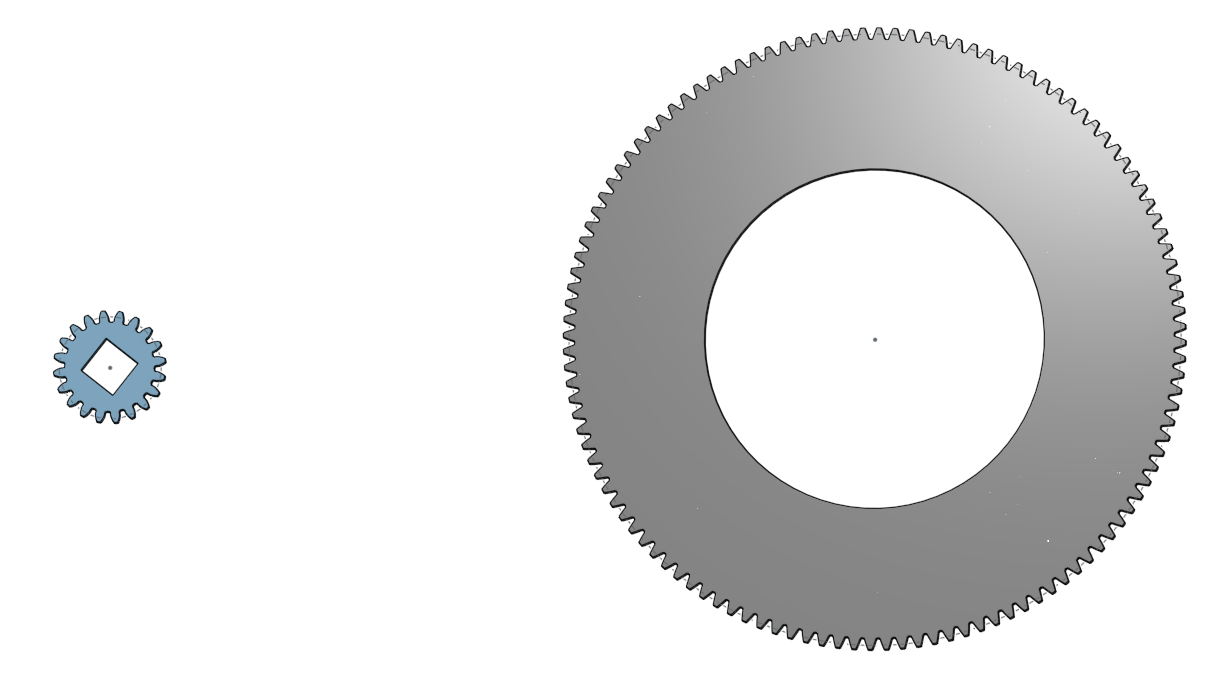
\includegraphics[width=10cm]{gears.png}
		\caption{Dimensionnement des engrenages}
	\end{figure}
	
	\newpage
	
	\subsubsection{Réalisation}
	
	Pour monter les éléments, on choisit de coller simplement l'engrenage à la bibine (avec le cercle central permettant d'alligner)
	
	Pour monter l'engrenage au moteur, on design une pièce intermédiaire qui mermet à la fois de maintenir l'engrenage (par une extrusion carrée qui correspond à la découpe carré dans l'engrenage) et de bloquer la rotation par rapport à l'axe du moteur pour que celui-ci puisse entraîner l'engrenage.
	
	\begin{figure}[h]
		\centering
		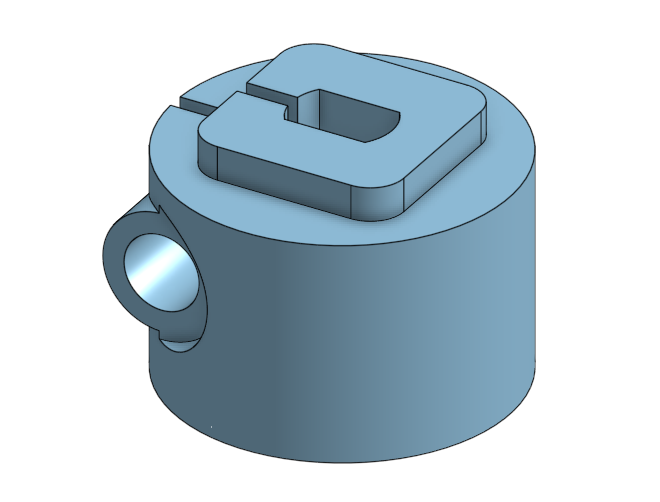
\includegraphics[width=10cm]{motor_holder.png}
		\caption{Model de la jonction moteur-engrenage}
	\end{figure}
	
	Pour maintenir la bobine en position pour l'engrenage, on a utilisé la découpe laser pour créer un bobineur (dont les models ont été obtenus \href{https://cults3d.com/fr/mod%C3%A8le-3d/outil/coudnicolas-4a7a}{ici})
		
	

\end{document}